\documentclass[12pt]{article}
\usepackage[utf8]{inputenc}
\usepackage[slovene]{babel}

\usepackage{hyperref}
\usepackage{listings} % za naslovnico
\usepackage{amsthm}
\usepackage{amsmath, amssymb, amsfonts}
\usepackage{graphicx}
\graphicspath{ {.} }
\usepackage{subcaption} % za side-by-side slike
\usepackage[
top    = 2.cm,
bottom = 2.cm,
left   = 2.cm,
right  = 2.cm]{geometry}

\usepackage{footnote}
\makesavenoteenv{tabular}
\title{Seminarska naloga ITAP - 2.del}

\begin{document}
    
\author{Vito Rozman}
\date{\today}
\maketitle


\textbf{Krčenje razsežnosti} 
Pri manjšanju razsežnosti podatkov sem uporabil štiri pristope, varianca, t-test, 
relief in pomembnost \emph{rf}. Za vsako od teh metod sem razvrstil spremenljivke od naj 
pomembnejše do najmanj pomembne. Nato sem testiral natančnost na testni množici, 
v odvisnosti od števila spremenljivk. Model, ki sem ga uporabil za učenje je bil \emph{rf}, 
z nastavitvijo parametra $ntree=100$. Poskusil sem tudi metodo \emph{pca}.

Za vsako napovedovanje območja (gozdovi, pozidano) sem natreniral model z vsemi značilkami in preveril 
natančnost na testni množici, tako sem dobil željeno natančnost, ki sem jo hotel doseči z čim manj
značilkami. Nato sem na podlagi zgoraj izbraih metod primerjal natančnost 
modelov, kjer sem dodajal vedno več značil (seveda od najbolj pomebne do najmanj). Tista metoda, ki 
je z najmanj značilk dosegla mejno natačnost, je bila izbrana za najboljšo.

\textbf{Izbira metode}
Izbiro najpomebnejših sprmenljivk pri napovedovanju gozdov sem naredil na podlagi 
\emph{relief} metode, pri napovedovanju pozidanega območja pa z \emph{t-test}-om in sicer
glede na vredost statistike.




\vspace{0.5cm}

\textbf{Glavne komponente} 
\begin{itemize}
    \item Napovedovanje gozdov: B02, B03, B12, B08, NDWI, NDBI, NDVI
    \item Napovedovanje pozidanega območja: B09, B8A, NDVI 
\end{itemize}

\begin{center}    
    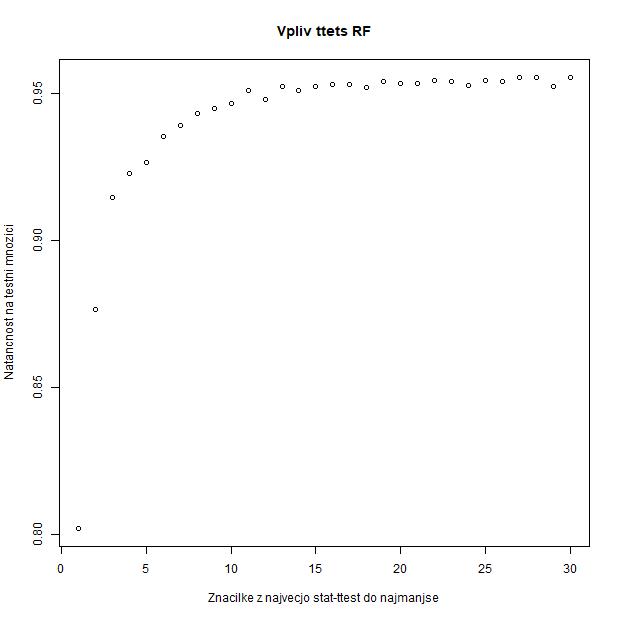
\includegraphics[width=8.5cm, height=8.5cm]{ttestRF.jpg}
    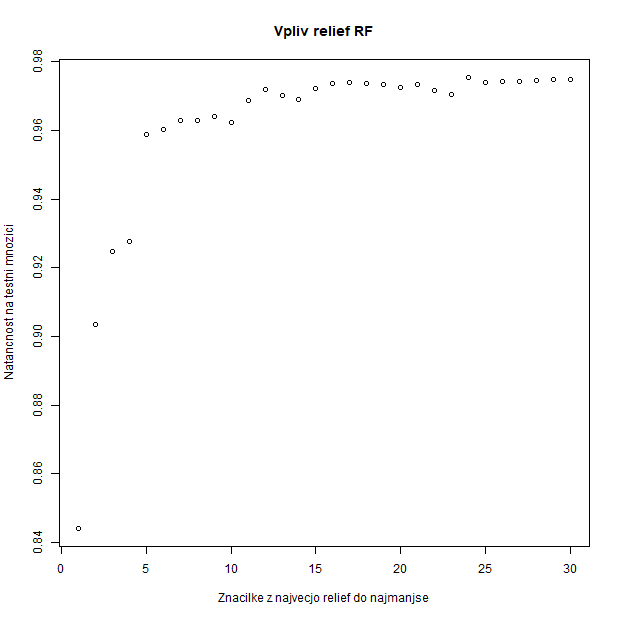
\includegraphics[width=8.5cm, height=8.5cm]{relRF.jpg}
\end{center}




\end{document}